\documentclass{jarticle}
\usepackage{robomech}
\usepackage{graphicx}
\usepackage{amsmath}
\usepackage{bm}
\usepackage{here}
\usepackage{siunitx}

\begin{document}
\makeatletter
\title{空中作業を行う多関節飛行ロボットのための遠隔操縦システムの開発}
{}
% {―日本語副題:ゴシック体・12pt(欧文Arial・12pt)―}
{Development of a manipulation-based teleoperation system for an articulated aerial robot}
{}
% {-English Subtitle: Times New Roman, 10pt-}

\author{
\begin{tabular}{ll}
 \hspace{1zw}○ 学\hspace{1zw}金子輝太朗 (東京大)& 正\hspace{1zw} 趙漠居(東京大) \\\hspace{1zw} 杉原淳一朗(東京大)& \hspace{1zw} 杉原和輝(東京大)\\
 \hspace{1zw} 小塚陽希(東京大)& \hspace{1zw} 西尾卓純(東京大)\\ \hspace{1zw} 長藤圭介(東京大)& \hspace{1zw} 中尾政之(東京大)
%  \hspace{1zw}学\hspace{1zw}東京 学(西大)& [日本語著者名:明朝体10pt]\\
 % ※協賛・後援団体の会員資格で発表される場合は「正・学」は不要です。
 \end{tabular}
 % &\\
 \vspace{1zh} \\
 \begin{tabular}{l}
{\small Kotaro KANEKO, University of Tokyo, kaneko@hnl.t.u-tokyo.ac.jp}\\
 {\small Moju ZHAO, University of Tokyo, }\\

 {\small Junichiro SUGIHARA, University of Tokyo,}
 ~{\small Kazuki SUGIHARA, University of Tokyo}\\
 {\small Haruki KOZUKA, University of Tokyo,}
 ~{\small Takuzumi NISHIO, University of Tokyo}\\
 {\small Keisuke NAGATO, University of Tokyo,}
 ~{\small Masayuki NAKAO, University of Tokyo}\\
\end{tabular}
}
\makeatother

\abstract{ \small 
Recently, robot teleoperation has been researched.
This is suitable for performing tasks in environments that are inaccessible to humans.
In particular, remote control of aerial robots is used for high-place work.
Currently, mainly used aerial robots are multirotors with manipulators attached to them.
Such robots can replace humans in high-place work.
However, they have not been able to approach locations in a cluttered environment.
One solution to this problem is to use an articulated aerial robot.
Articulated aerial robots have redundant Degrees-of-Freedom(DOFs), squeeze in the cluttered environment by changing the shape and approach the end effector.
To remotely control an articulated aerial robot, it is necessary to control the robot's multiple DOFs, such as joints and positions.
However, it is difficult for conventional devices to simultaneously control these DOFs. 
A device suitable for remote control of articulated aerial robots is needed.
To solve this problem, we propose a floating-based device with a skeleton similar to that of an articulated aerial robot.
Beside, some tasks require the robot to exert force with its end effector, and external forces such as the reaction force and friction from the environment can make the robot's flight unstable.
It is desirable for the robot to control forces autonomously and stabilize its flight.
Only using the thrust scalar to compensate for the external forces has the limitation, thereby we also focus on the thrust direction, and introduce a vectoring apparatus that can change the direction. 
In this study, we propose an autonomous control method that achieves both end effector force exertion and flight stabilization by controlling the vectorable thrust force.
Finally, we verify the proposed methods by conducting wall-cleaning experiments using an articulated aerial robot with vectoring.
}

\date{} % 日付を出力しない
\keywords{aerial robot, teleoperation, aerial manipulation, force control, optimization planning}

\maketitle
\thispagestyle{empty}
\pagestyle{empty}

\small
\section{序論}
ロボットの遠隔操縦は以前から研究されている\cite{survey_on_teleop}.遠く離れた場所や人が立ち入ることができない場所で作業を行うためには,ロボットの遠隔操縦は有用である.
これまでは主にロボットアームや人型ロボットの遠隔操縦が研究されている\cite{survey_on_humanoid}.これらのロボットは手先の多自由度が必要とされるタスクに適している.
しかし、これらの研究はベースが固定もしくは地上での移動に限られている。一方空中での作業には飛行ロボットが用いられる.
飛行ロボットの遠隔操縦についても研究がなされているが,関節を持たない自由度の低いロボットに限定されている.
狭い場所や奥まった場所など,周囲に障害物がある状態でタスクを実行する場合には,身体の多自由度が必要とされる.
身体に多自由度を有する飛行ロボットとして,多関節飛行ロボットがZhaoら\cite{hydrus_xi}によって提案されている.
このようなロボットは機体を変形させることができるため,障害物を回避して手先をアプローチさせることができる.
従来の多関節飛行ロボットのシステムでは,ロボットの持つ浮遊する基部の自由度と,関節の自由度を同時に操縦することができず,遠隔操縦によってタスクを実行することが難しい.
そこで本研究では,図1のような空中で作業を行うための,多関節飛行ロボットの遠隔操縦システムの構築を目指す.
\begin{figure}[tb]
    \centering
    \includegraphics[width=1.0\columnwidth]{figs/experiment_operator_image.eps}
    \caption{Articulated aerial robot controled by operator}
    \label{fig:total_system_image}
\end{figure}

マルチロータと呼ばれるような関節を持たない飛行ロボットの遠隔操縦については研究がすすめられている.
Macchiniら\cite{drone_hand_haptics}は,操縦者の手の動きによってマルチロータを操縦できるシステムを提案している.
このシステムではマルチロータ周辺に障害物がある時,操縦者の手に振動をフィードバックすることで障害物の存在を知らせ,より容易な遠隔操縦を実現している.
% Yuら\cite{gaze_control}は,操縦者の視線移動によるマルチロータの遠隔操縦を提案している.
% このシステムではあらかじめ決められた視線移動のジェスチャーによってマルチロータの移動を操縦する.
この手法では飛行ロボットを質点として操縦することができるが,関節を持つロボットを操縦する場合では,これらのシステムに関節角を操縦するための入力を同時に組み込むことが難しい.

通常の多リンク構造ロボットの遠隔操縦についても多くの研究がなされている.
Schuwarzら\cite{nimbro}は双腕の多リンクロボットを遠隔操縦するシステムを提案している.
% 操縦者は,操縦対象と同じ構造のアームを操作する.
操縦者から入力された手先の6自由度を実現するよう逆運動学を解き,ロボットに指令する.
この手法は基部の固定されたロボットでは有用であるが,基部が浮遊している飛行ロボットでは手先の位置と姿勢に対し基部も自由度を持つため,逆運動学的に関節角を決定することが難しい.

% 多関節飛行ロボットは基部が浮遊する飛行ロボットの特性と,関節を持つ多リンク構造ロボットの特性を併せ持つ.
% このロボットを両手で遠隔操縦するためには,先行研究で提案された手法を統合するだけでは不十分である.
そこで本研究では,操縦対象のロボットと相似な骨格を持つ浮遊型の操縦デバイスを提案する.
% 提案するデバイスを用いることで,多関節飛行ロボットの持つ多自由度をすべて両手で同時に操縦することができる.
% また,手元でロボットの取る姿勢を表現できるため,作業を行うためにどのような操作が必要であるかを操縦者が認識しやすくなる.

ロボットが作業を行う上では,ロボットの発揮する手先力を制御することが重要である.基部の固定された多リンク構造ロボットでは関節トルクを制御することで目標の手先力を実現する.
Mahvashら\cite{Mahvash}は,操縦者がロボットの手先力を操縦するために,ロボットの関節トルクを制御することに加え,関節に発生する摩擦力をフィードフォワード的に補償するシステムを提案している.
一方,飛行ロボットでは基部が固定されていないため,推力を制御することで手先力を実現する.その際に,外力を補償し飛行を安定化させる必要がある.
Alexisら\cite{Alexis}は,エンドエフェクタを環境と接触させた状態で飛行ロボットを制御する手法を提案している.
この手法では,各ロータの発揮する推力の大きさを制御対象としている.しかし推力の大きさだけでなく,向きも制御対象に含めるほうが,より安定して強い力を発揮することができる.
% そこで本研究では,ロータが偏向可能であるとみなすことで,目標の手先力を実現し飛行を安定化させる.Bodieら\cite{Bodie}は,偏向可能なロータをもつ飛行ロボットを用いることで,安定した環境との接触を実現している.
また,杉藤ら\cite{sugito}は,偏向可能なロータを持った飛行ロボットを用いての空中作業の制御手法を提案している.
この研究では偏向可能なロータを用いることで手先外力の補償を達成している.本研究ではこれを発展させる形で,発揮する手先力を推定し,制御することを目指す.

% \begin{figure}[tb]
%     \centering
%     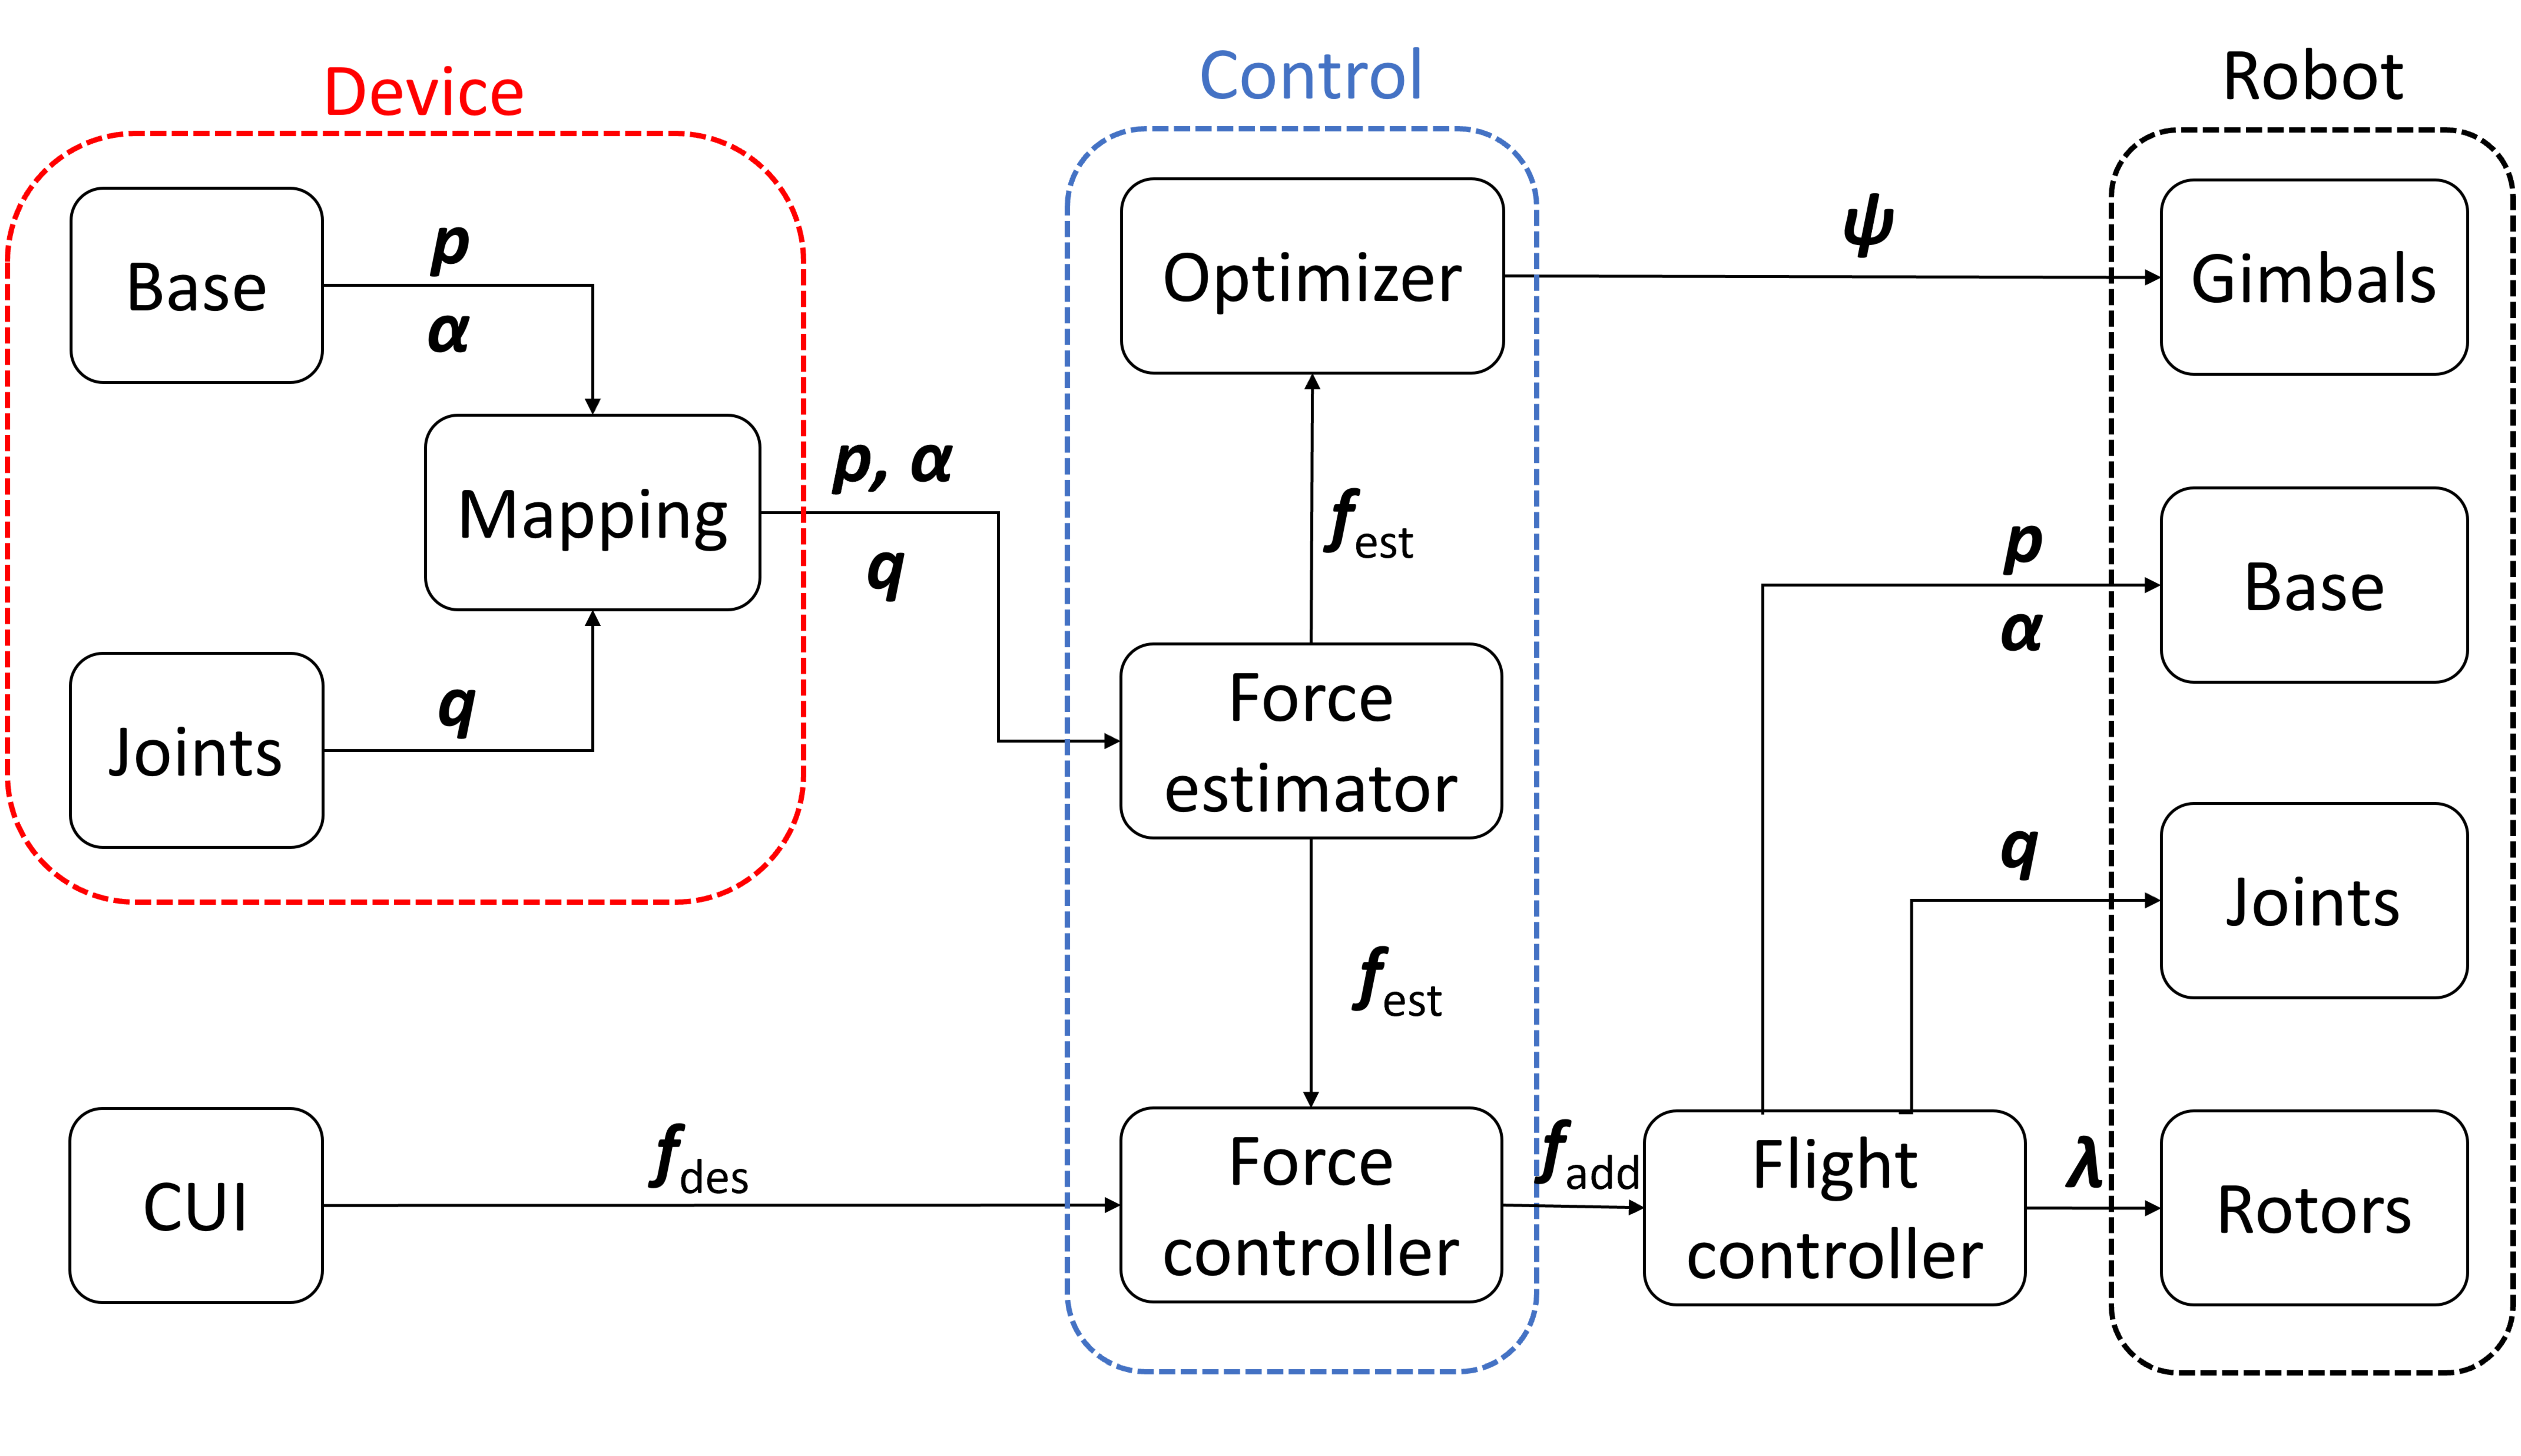
\includegraphics[width=0.6\columnwidth]{figs/system_block.eps}
%     \caption{Diagram of the remote control system, $\bm{p}$ is position, $\bm{\alpha}$ is orientation, $\bm{q}$ is joint angles, $\bm{\psi}$ is yaw angles of rotors (gimbal angles),
%     $\bm{\lambda}$ is thrusts fo rotor, $\bm{f_{des}}$ is desire end-effector force, and $\bm{f_{est}}$ is estimated end-effector force}
%     \label{fig:diagram_of_system}
% \end{figure}

% 本研究で提案する遠隔操縦システムの全体図は図2である.
本研究のコントリビューションを要約すると以下の3つである.
\begin{itemize}
\item 多関節飛行ロボットの持つ浮遊ベースと関節の自由度を同時に操縦するための,ロボットと相似な骨格を持つ浮遊型の遠隔操縦用デバイスを提案する.
\item 多関節飛行ロボットが作業を行う際,目標の手先力の発揮と飛行の安定化のための,推力ベクトルの制御手法を提案する.
\item 多関節飛行ロボットの遠隔操縦による壁面清掃実験によって,提案する遠隔操縦システムの有用性を実証した.
\end{itemize}
% 我々の知る限りでは,本研究は多関節飛行ロボットを遠隔操縦し空中作業を行った初めての取り組みである.

% 本論文は以下のように構成される.第二章では,多関節飛行ロボットを遠隔操縦するためのデバイスについて述べる.
% 第3章では,ロボットの飛行を安定させつつ,目標の手先力を発揮するための自律飛行制御について述べる.
% 第4章では,本研究で提案したデバイスと自律制御を用いて行った壁面清掃実験の結果と考察を述べる.
% 第5章では,結論と今後の展望を述べる.

\section{デバイスの設計}
\subsection{デバイスの必要機能}
本研究では,操縦者が両手で多関節飛行ロボットを操縦するためのデバイスの開発を目指す.
人間の手は,指を用いずに質点として考えた場合,位置と姿勢の6自由度を表現でき,両手では12自由度である.
一方多関節飛行ロボットは,基部の位置と姿勢について6自由度を持つ.
また関節一つにつき,pitch,yaw方向の2自由度を持つ.ただしroll方向については機体の骨格形状の変形にはかかわらないため考慮しない.
よって人間が両手で操縦できるリンク数は以下のように計算される.
\begin{eqnarray}
    6 + (n-1) \times 2 &\leq& 12 ,\\
    n_{max} &=& 4 .
\end{eqnarray}
そこで本研究では4リンクで構成され,関節にpitch,yaw方向の2自由度をもつハードウェアを構築する.そして基部となるリンクの位置と姿勢の6自由度を入力として受け取る.
デバイスの構造は図\ref{fig:avatar_image}のようである.
また,操縦者がデバイスで入力することができる形状は,必ずしもロボットが実現できる形状とは限らない.
そして操縦者の手の可動範囲はロボットの移動可能な範囲にくらべ狭い.そのため,操縦者の入力値からロボットの指令値への適切なマッピングが必要となる.
\begin{figure}[tb]
    \centering
    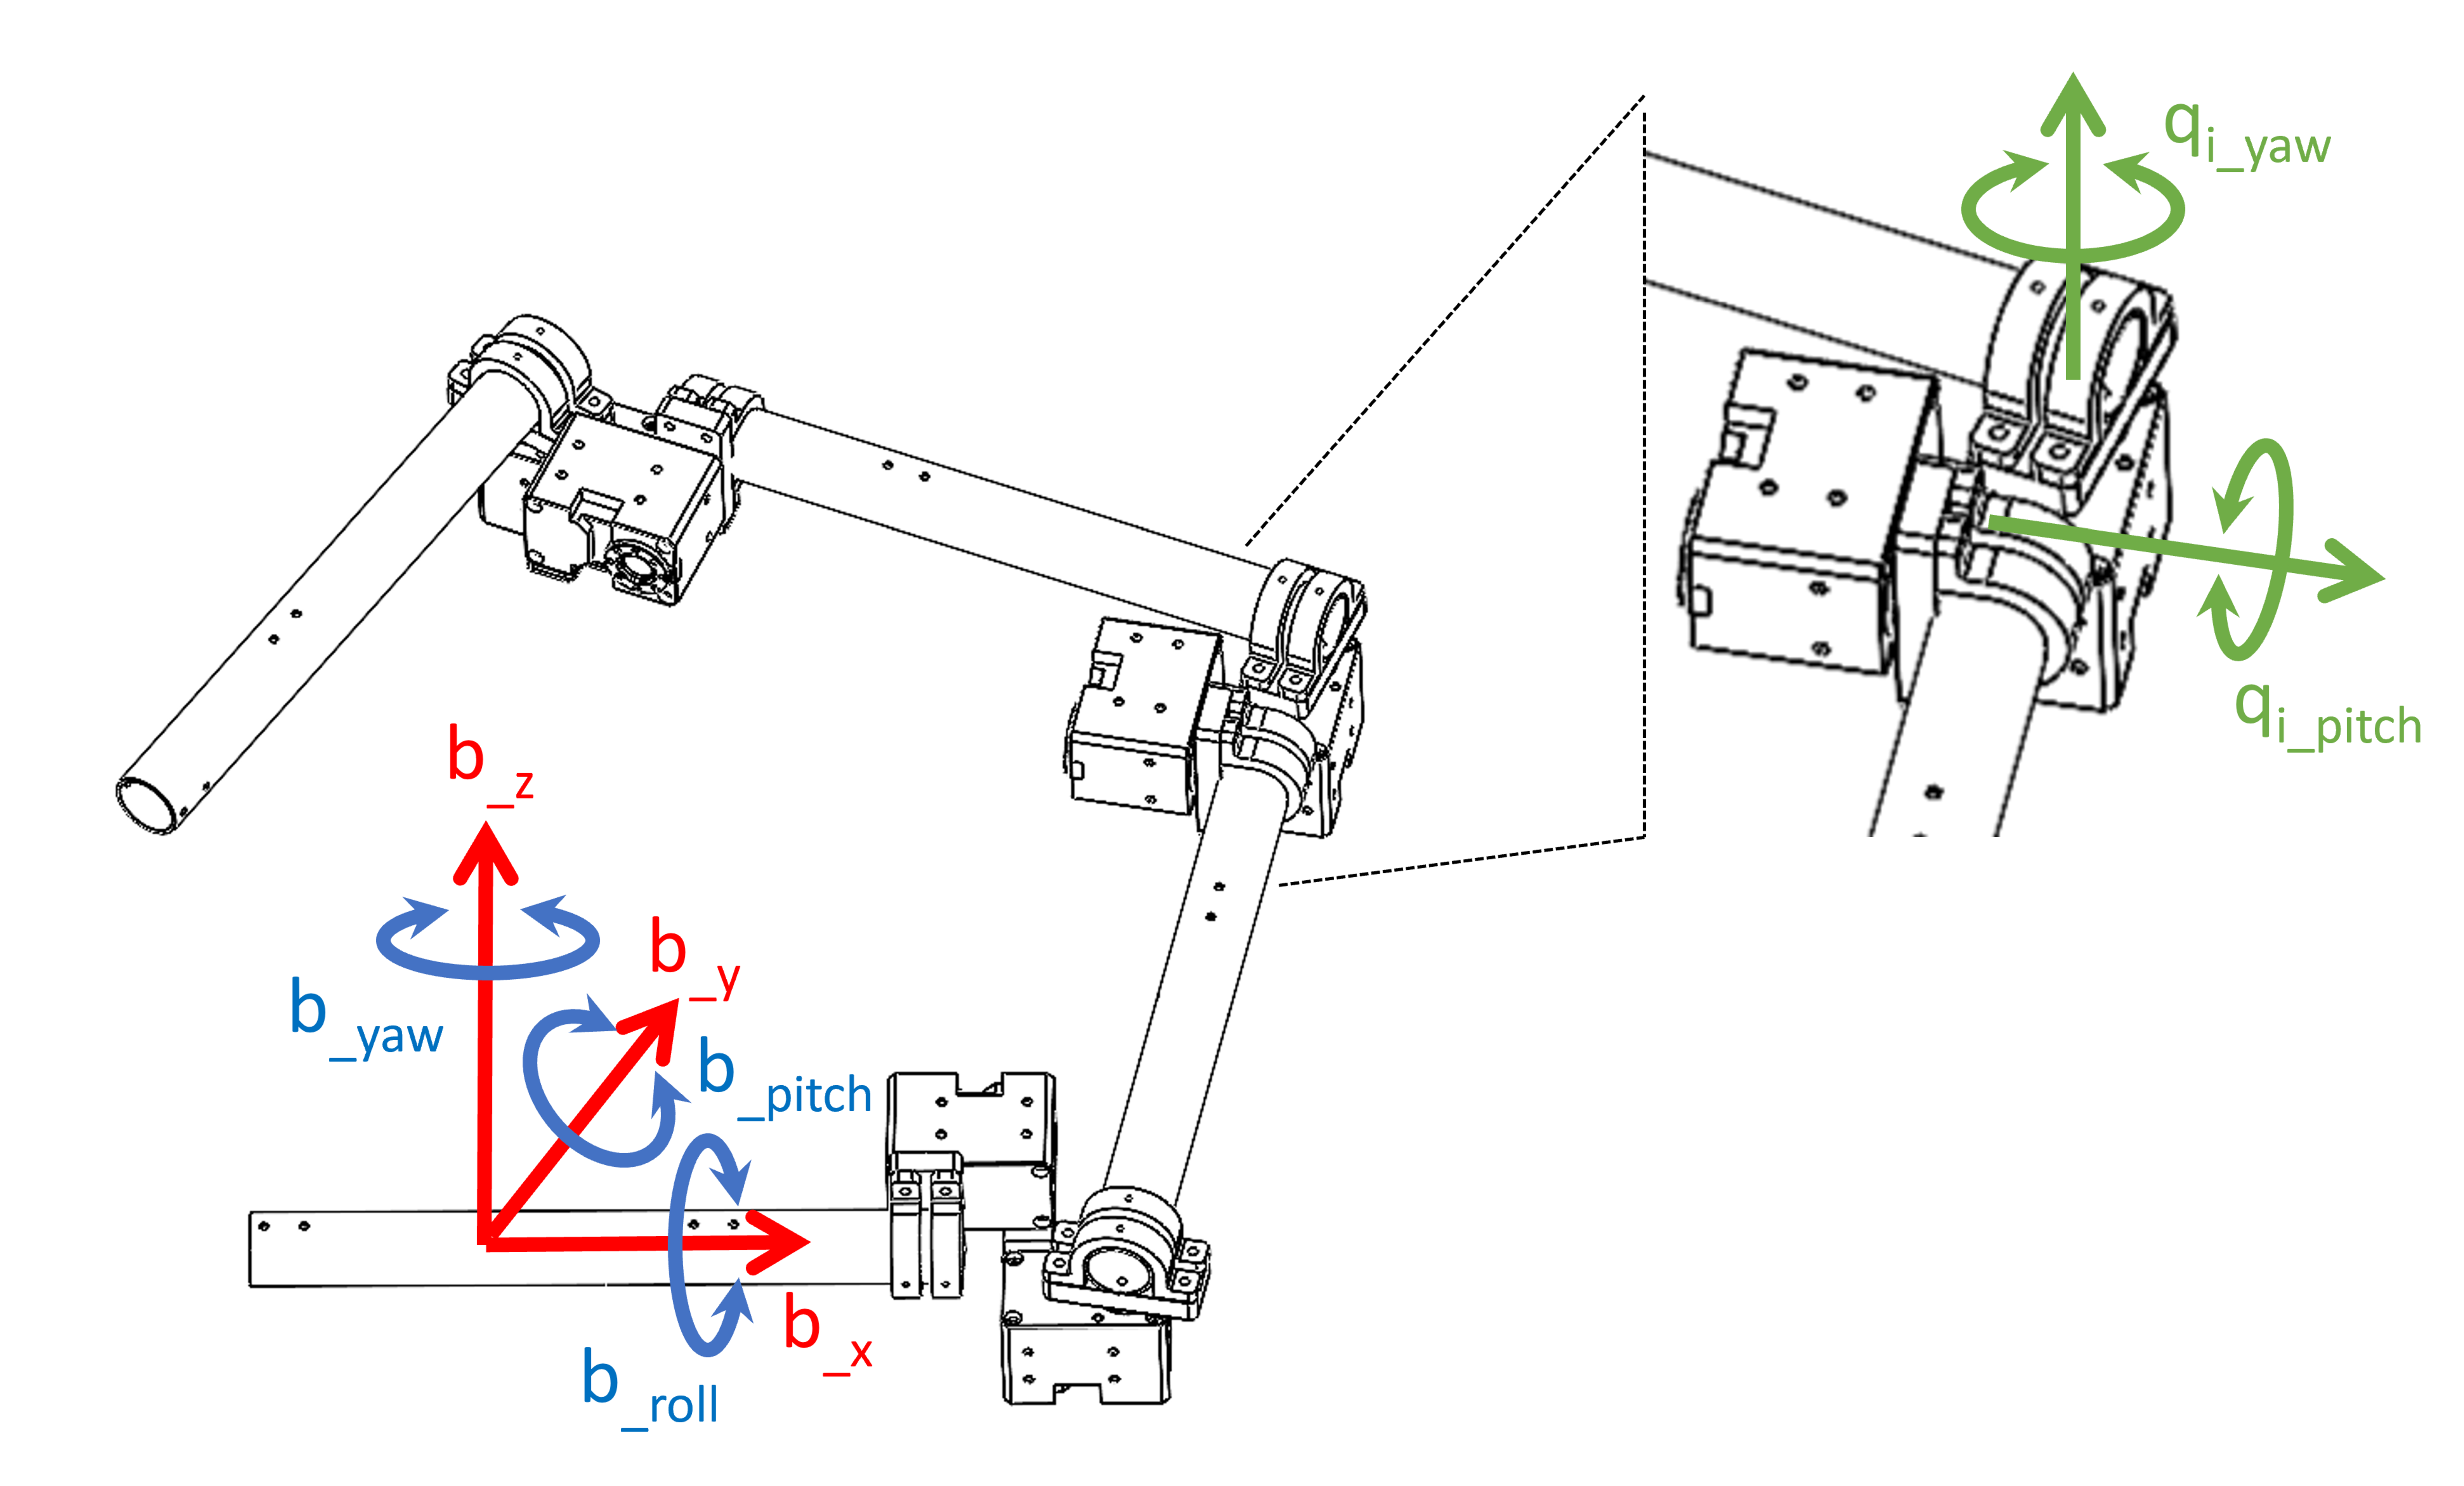
\includegraphics[width=0.6\columnwidth]{figs/device_concept.eps}
    \caption{Design of the device for controlling articulated aerial robot}
    \label{fig:avatar_image}
\end{figure}

\subsection{マッピング}
関節角について,デバイスの関節の角度を,対応するロボットの関節角への入力とする.
その際,ロボットの取ることができる限界角と,デバイスの限界角は異なるため,ロボットの限界角の範囲内に丸めて指令する.
また,ロボットの関節の自由度がデバイスの関節の自由度より小さい場合には,対応しない関節をロックし,入力を受け取らない.
ベースリンクの姿勢については,操縦者がデバイスとロボットの対応がわかりやすいように,ワールド座標におけるデバイスの姿勢を,ワールド座標におけるロボットの姿勢の指令値とする.
ベースリンクの位置については,デバイスの移動した量をスケーリングして,ロボットの目標移動量とする.
スケーリングには,タスク実行場所への移動の容易さと,細かなタスクを実行する容易さのトレードオフが存在する.行うタスクによって適切にスケールの値を決定する必要がある.
% \begin{figure}[tb]
%     \centering
%     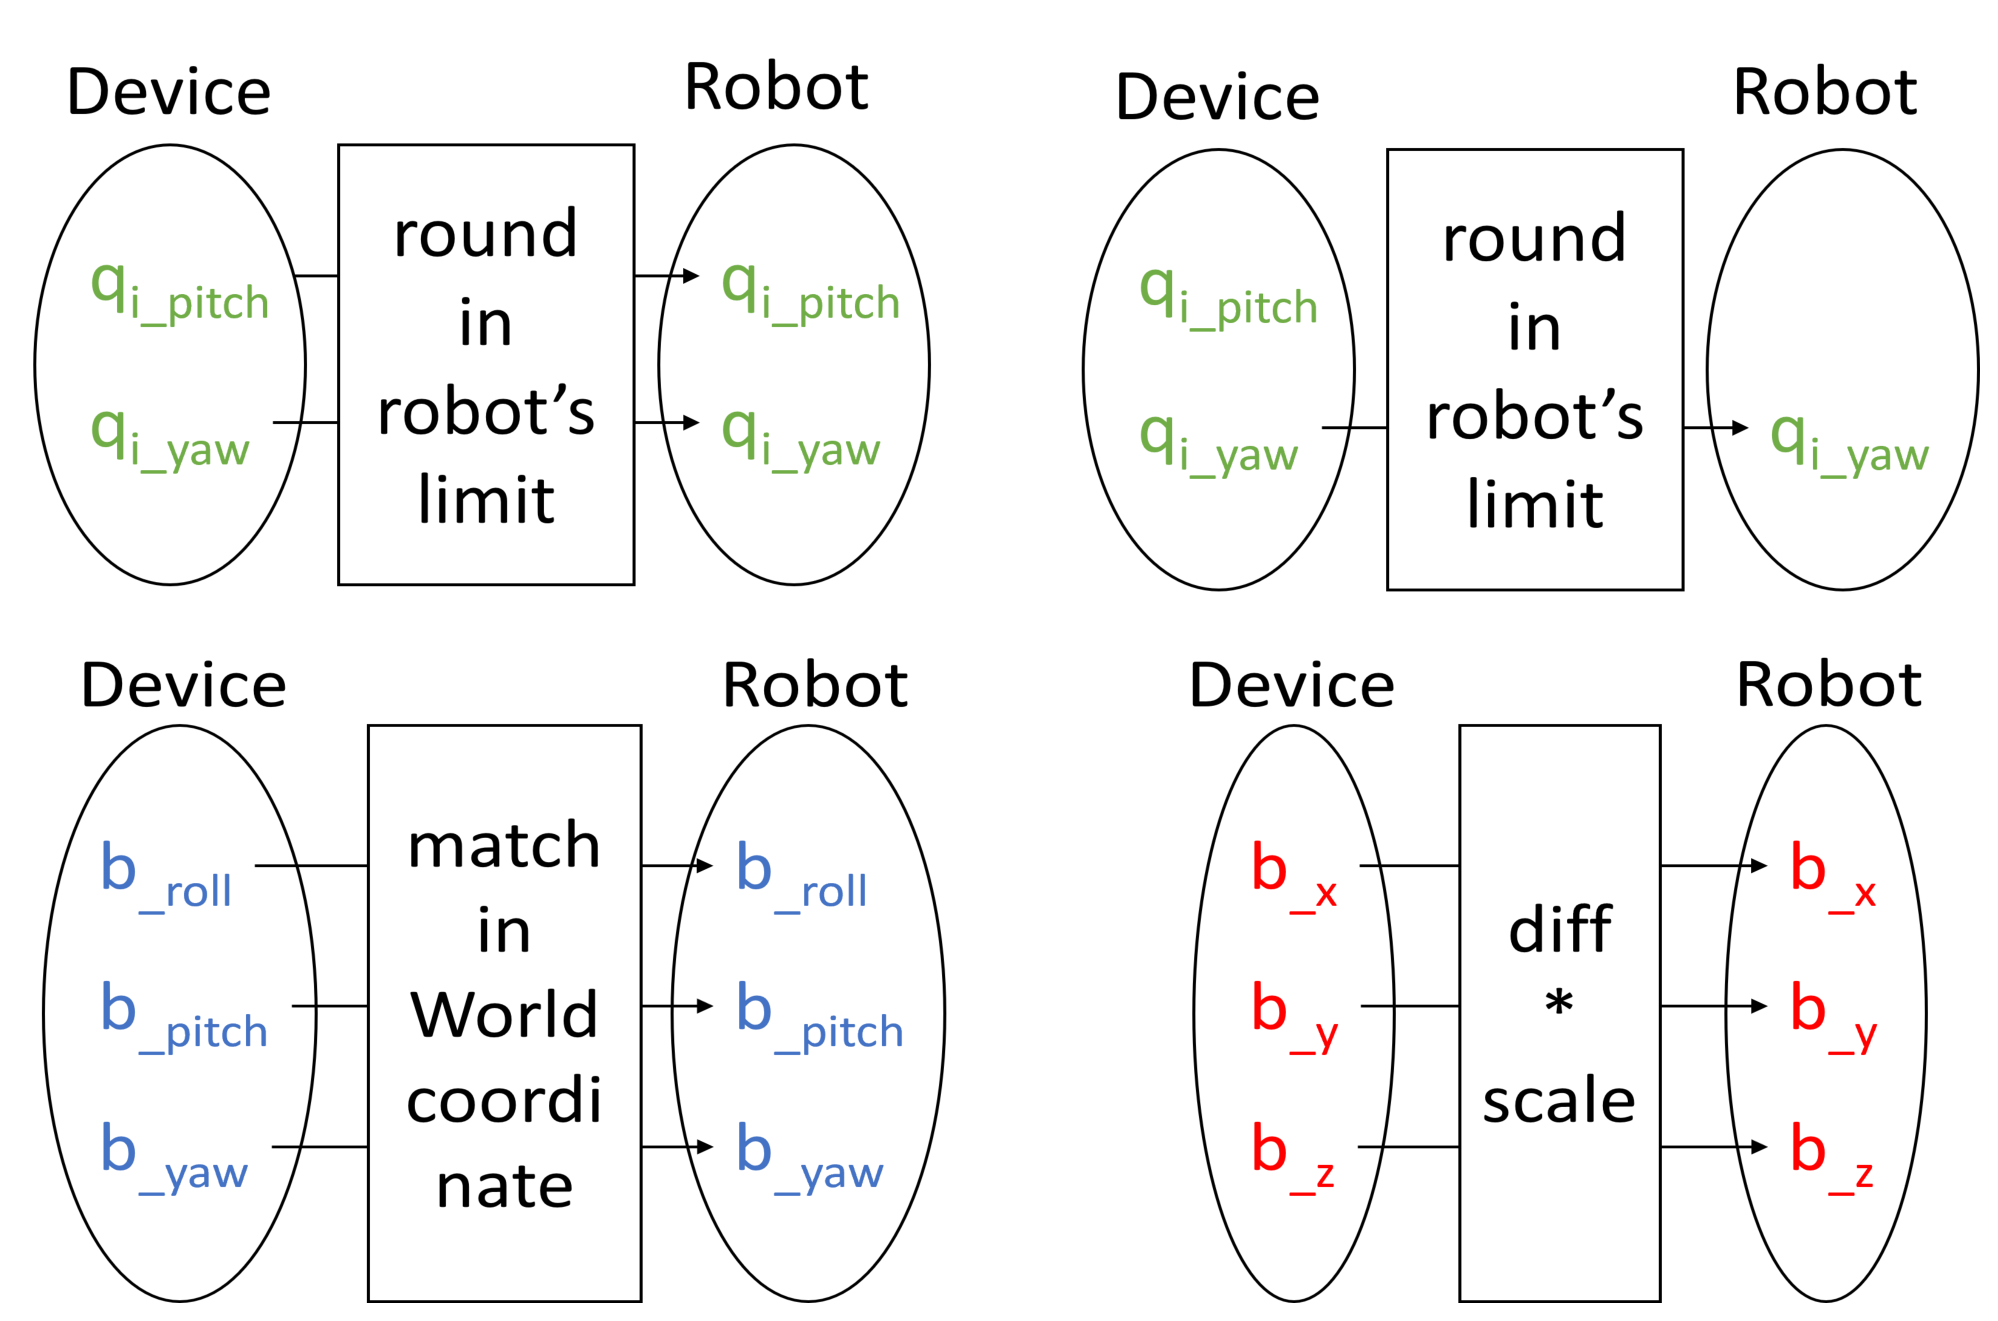
\includegraphics[width=0.6\columnwidth]{figs/mapping.eps}
%     \caption{Top-Right:Mapping to 2 DOFs robot's joint, Top-Left:Mapping to 1 DOF robot's joint
%     Bottom-Right:Mapping of base attitude, Bottom-Left:Mapping of base position}
%     \label{fig:mapping}
% \end{figure}

\section{補助自律制御}
本章では遠隔操縦中にタスクの実行を補助する自律制御について述べる.
タスクを行う際には,ロボットはエンドエフェクタに反力や摩擦力を受ける.
その外力を補償し飛行を安定させる必要がある.
また,円滑にタスクを実行するためには,エンドエフェクタの力を制御することが望ましい.
ロータの偏向角と推力を制御することで,飛行を安定させ,エンドエフェクタの目標力を発揮することを目指す.
本研究では,操縦対象のロボットとしてZhaoら\cite{hydrus_xi}の開発したHYDRUS\_XIを用いる.
% このロボットは4リンクで構成され,ロータに偏向角の1自由度を持つ多関節飛行ロボットである.
偏向角に自由度を持つ多関節飛行ロボットとしては最小の構成であるため,このロボットを用いる.

\subsection{ロボットモデル}
\begin{figure}[tb]
    \centering
    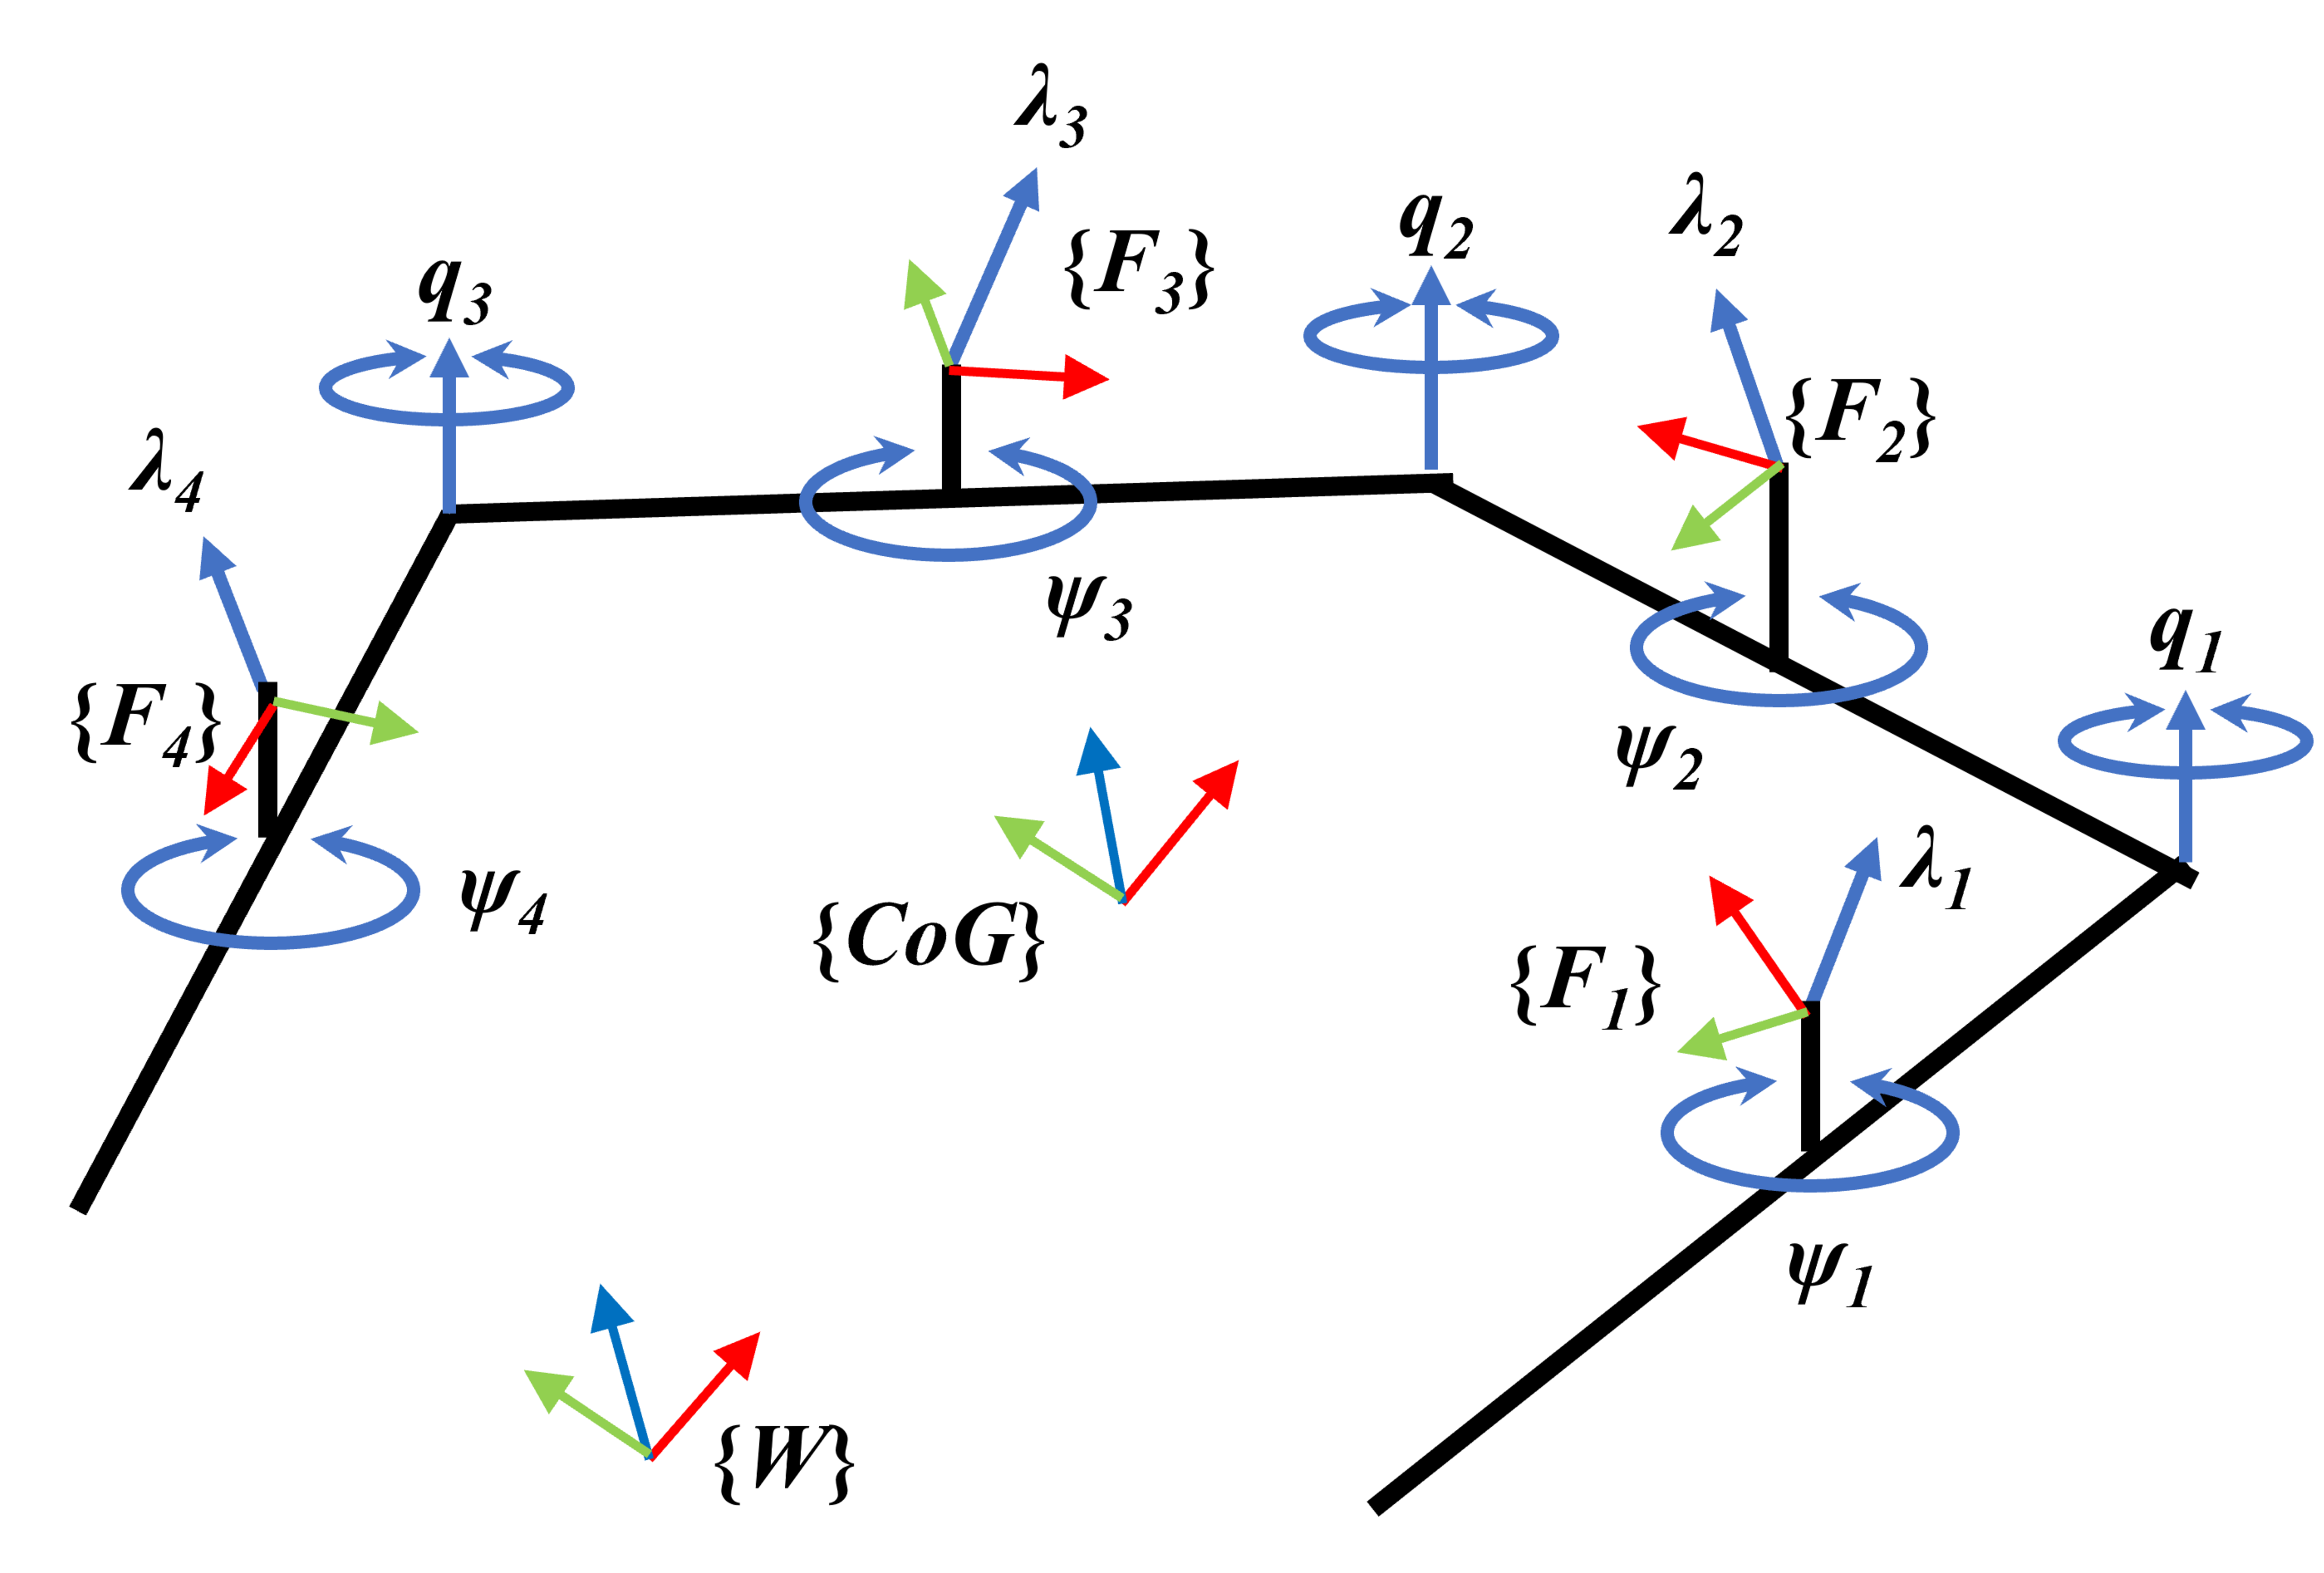
\includegraphics[width=0.6\columnwidth]{figs/hydrus_xi_kine_frame.eps}
    \caption{Kinematics model of the multilinked structure of the robot.
    The frame $\{W\}$ is an inertial reference frame where the gravity is along the z axis.
    The frame $\{CoG\}$ have the origin at the center-of-mass of the whole model.
    The frame $\{F_i\}$is attached to each rotor mount, and the thrust force $\lambda_i$ yields along the z axis of $\{F_i\}$.
    }
    \label{fig:hydrus_xi_Frame}
\end{figure}

はじめに運動モデルについて述べる.
重心座標系において,各ロータによって発揮される力とトルクは以下のように書くことができる.
\begin{equation}
    \bm{f}_i = \lambda_i R(\bm{q},\bm{\psi}) \bm{b} ,
\end{equation}
\begin{eqnarray}
    \bm{\tau}_i &=& \bm{p}(\bm{q},\bm{\psi}) \times \bm{f}_i + \kappa_i \bm{f}_i , \\
    &=& \lambda_i \{\bm{p}(\bm{q},\bm{\psi}) + \kappa_i E_{3\times3}\} R(\bm{q},\bm{\psi}) \bm{b} ,
\end{eqnarray}
% ただし$i={1,2,3,4}$である. 
% $\bm{q}=(q_0\ q_1\ q_2)^T$はロボットの関節角である.
% $\bm{\psi}=(\psi_0\ \psi_1\ \psi_2\ \psi_3)^T$はロータの偏向角である.
$R(\bm{q},\bm{\psi})$ and $\bm{p}(\bm{q},\bm{\psi})$は重心座標系$\{CoG\}$でのロータ座標系$\{F_i\}$の回転行列と位置のベクトルである.
$\bm{b}$は単位ベクトル$[0 ~ 0 ~ 1]^T$であり,$\kappa_i$はロータの抗力係数である.
% $E_{3\times3}$は$3\times3$の単位行列である.

この式より,レンチから推力へのアロケーションは以下のように与えられる.
\begin{equation}
    \left(\begin{array}{c} \bm{f} \\ \bm{\tau} \end{array} \right) = \sum_{i=1}^{4} \left( \begin{array}{c} \bm{f}_i \\ \bm{\tau}_i \end{array} \right)
    = Q(\bm{q},\bm{\psi}) \bm{\lambda} ,
\end{equation}
ただし$Q(\bm{q},\bm{\psi}) = \left( \begin{array}{c} Q_{trans} \\ Q_{rot} \end{array}\right)$がアロケーション行列である.
$Q_{trans}, Q_{rot} \in \mathcal{R}^{3\times4}$は並進と回転についてのアロケーション行列である.

関節の動きは十分に遅いため,各制御周期ではロボットは剛体であるとみなすことができる.よって重心座標でのロボットの運動方程式は以下のように表すことができる.
\begin{equation}
    \label{equ:EOM_trans}
    m(\ddot{\bm{r}} + \bm{g}) ~=~ ^{\{W\}}R_{\{CoG\}} \, Q_{trans}(\bm{\psi},\bm{q})\bm{\lambda} ,
\end{equation}
\begin{equation}
    \label{equ:EOM_rot}
    I \dot{\bm{\omega}} ~+~ \bm{\omega} \times I \bm{\omega} ~=~ Q_{rot}(\bm{\psi},\bm{q})\bm{\lambda} ,
\end{equation}
ただし$\bm{r}$と$^{\{W\}}R_{\{CoG\}}$はワールド座標系$\{W\}$における重心座標系$\{CoG\}$の位置ベクトルと回転行列である.
$\bm{\omega}$は重心座標系$\{CoG\}$の角速度である.
% $I$は順運動学から計算されるロボットの慣性テンソルである.

% タスクの実行中,ロボットはほぼ水平であると仮定できるため,角速度について
% $\dot{\bm{\alpha}} \approx \bm{\omega}$
% と近似できる.ただし$\bm{\alpha}$はワールド座標系$\{W\}$での重心座標系$\{CoG\}$のオイラー角である.
% よって式\ref{equ:EOM_rot}は以下のように書き換えられる.
% \begin{equation}
%     I \ddot{\bm{\alpha}} ~+~ \bm{\omega} \times I \bm{\omega} ~=~ Q_{rot}(\bm{\psi},\bm{q})\bm{\lambda} .
% \end{equation}

\subsection{飛行の安定化}
飛行ロボットが空中で作業を行う場合,環境から及ぼされる外力により飛行の安定性が低下しうる.
本項では飛行の安定性の評価方法と,環境と接触した状態で飛行を安定させる制御手法について述べる.

\subsubsection{飛行の安定性の評価}
本研究では Parkら\cite{FCTMin}が提案する Feasible Control Torque Minimum の値を,飛行安定性の指標として用いる.
これはロボットが発揮しうるトルクの最小値である.
ある時点でのロボットの関節角$\bm{q}$,ロータのyaw角$\bm{\psi}$に対して,各ロータの推力$\lambda_i$を$\lambda_{max} > \lambda_i > 0$で動かした際,
発揮されるトルク$^\text{\{C\}}\tau(\textbf{\textit{q}},\bm{\psi})$は3次元トルク空間上に,以下で定義される多面体$\nu_T$を形成する.
\begin{equation}
    \begin{split}
    \nu_T ~:=~ \Big\{& ^\text{\{C\}}\tau(\bm{q},\bm{\psi}) \in \mathcal{R}^3 | \\
    &^\text{\{C\}} \tau(\bm{q},\bm{\psi}) = \sum_{i=0}^{3} \lambda_i\bm{\nu}_i(\bm{q},\bm{\psi}),  \lambda_{max}>\lambda_i>0   \Big\}
    \end{split}
\end{equation}
この多面体を Feasible Control Torque Convex と呼ぶ.
$\nu_T$に内接する,原点を中心とする球の半径は,ロボットが発揮しうる任意方向へのトルクのうち最小のものとなる.
これが Feasible Control Torque Minimum($\tau_{min}$)である. 
$\tau_{min}$が大きいほど,任意の方向にトルクを発揮できるため,環境から及ぼされる外力に対してロバストで,飛行安定性が高いと言える.

\subsubsection{安定性の最大化}
前項で述べた最小トルク$\tau_{min}$を最大化することで,飛行を安定化させることを目指す.
本研究ではロータの向きの自由度を制御し,$\tau_{min}$を最大化する非線形最適化問題を解く.
その際にロボットのハード構成上考慮すべき制約条件が存在する.

\paragraph{ロータの向きの角度連続条件}
~ ロータの向きを制御するサーボモータの角速度には上限があるため,ある時刻$t+dt$でのyaw角$\psi_i(t+dt)$には以下の制約条件が存在する.
\begin{equation}
    \label{eq:angle_continuity}
    \psi_i(t)-\omega_{max}dt \leq \psi_i(t+dt) \leq \psi_i(t)+\omega_{max}dt
\end{equation}

\paragraph{推力範囲条件}
~ ロータには回転速度の上限が存在するため,発揮される推力にも上限$\lambda_{max}$が存在する.
加えて,ロータの回転方向は,時計回りか反時計周りのどちらかのみで用いることから,ロータの推力の範囲は以下のようになる.
\begin{equation}
    \label{eq:thrust_limit}
    0 \leq \lambda_i \leq \lambda_{max}
\end{equation}

% 環境からの外力を受ける状態では,発揮する推力が上限と下限に対し余裕を持つことが望ましい.
% ロボットはホバリングするために一定の推力を必要とするため,すべてのロータの推力が下限に接近することはない.
% そのため,推力ベクトルのノルム$|\bm{\lambda}|$を最小化することが,上限からの余裕を最大化することとなる.
% また,ホバリングのための推力を一部のロータのみで発揮すると,そのロータの推力は上限に接近してしまう.
% すべてのロータの推力が均等になることが,上限からの余裕を持つこととなるため,推力ベクトルの分散$\text{val}(\lambda) = \frac{1}{4} \sum_{i=0}^{3} \lambda_i^2$も最小化する.

この際,各ロータの推力ベクトルのノルムと分散を最小化することで,発揮推力が上下限に接近しないようにする.

\paragraph{機体姿勢角条件}
~ 機体が過度に傾いてしまうと,清掃用の手先を壁面にならわせることができなくなってしまう.そこで機体の姿勢角に以下の制約条件を課す.
ワールド座標系からみた,重心座標系の回転行列は以下のように表せる.
\begin{eqnarray}
    ^{\{W\}}R_{\{cog\}} = \left( \bm{e}_x \ \bm{e}_y \ \bm{e}_z\right) \\
    \bm{e}_z = (e_{z_x} \ e_{z_y} \ e_{z_z})^T
\end{eqnarray}
上式から機体の重心座標の傾きの制約条件は,機体姿勢角の上限$\alpha_{thresh}$を用いて,以下のように書ける.
\begin{equation}
    \label{eq:rot_const}
    \alpha = \arctan\left( \frac{\sqrt{e_{z_x}^2+e_{z_y}^2}}{|e_{z_z}|}\right) \leq \alpha_{thresh}
\end{equation}

\paragraph{外力補償条件}
~ ロボットは清掃作業中に,手先を押し付けた反力と,壁面に沿った方向の摩擦力を受ける.
この反力と摩擦力からなる外力は,先に述べた外力推定の手法から推定できる.
% 飛行を安定させるためにはこの外力を補償する必要がある.
% 機体のコンフィギュレーションと,発揮すべきレンチから,外力の補償のために必要な推力が求められる.
推定された外力を$\bm{f_{est}}$とすると,以下のような等式条件が存在する.
\begin{equation}
    \label{eq:force_comp}
    \mathcal{Q}\bm(\psi)\bm{\lambda} = \left(\bm{f}_{est}^T \quad 0 \right)^T
\end{equation}

\paragraph{非線形最適化問題による求解}
~ ロータの向き$\bm{\psi}$と推力ベクトル$\bm{\lambda}$を合わせた8次元の変数$[\bm{\psi},\bm{\lambda}]^T$を入力とし,目標レンチ$\bm{w}$を出力とする問題を考える.
そして得られたロータの向き$\bm{\psi}$を制御の目標値とする.
解くべき非線形最適化問題は以下である.
\begin{equation}
    \max_{(\bm{\psi}\bm{\lambda})} \quad \left(\frac{k_{norm}}{|\bm{\lambda}|} \right) + \left(\frac{k_{var}}{\text{val}(\bm{\lambda})} \right) + \left(k_{FCTmin}\tau_{min} \right)
\end{equation}
ただし,$k_{norm},k_{val},k_{FCTmin}$はそれぞれの重み係数である.
これに制約条件として式\ref{eq:angle_continuity},式\ref{eq:thrust_limit},式\ref{eq:rot_const},式\ref{eq:force_comp}を与える.

\subsection{手先の壁面への押し付け}
\subsubsection{手先の押し付け力の推定}
手先を押し付ける力を制御するためには,発揮している力を知る必要がある.
本研究ではLucaら\cite{wrench_est}の提案する外レンチ推定を用いることで,手先の押付力の反力を推定する.
運動量$\bm{p}$,速度$\bm{v}$,ロータから発揮される推力によるレンチ$\bm{w}$,実際に発生する外レンチ$\bm{w}_e$について,以下の等式が成立する.
\begin{equation}
    \dot{\bm{p}} ~=~ M\dot{\bm{\nu}} = J^T\bm{w} + \bm{w}_e - \bm{N}
\end{equation}
\begin{eqnarray*}
    M &=& \left( \begin{array}{rr} mE_{3\times3} & O_{3\times3} \\ O_{3\times3} & I \end{array} \right) ,~
    J = \left( \begin{array}{rr} R^T & O_{3\times3} \\ O_{3\times3} & E_{3\times3} \end{array} \right) \\
    \bm{N} &=& \left( \begin{array}{c} m\bm{g} \\ \bm{\omega}\times I\bm{\omega} \end{array} \right)
\end{eqnarray*}
% \begin{equation*}
%     M = \left( \begin{array}{rr} mE_{3\times3} & O_{3\times3} \\ O_{3\times3} & I \end{array} \right) 
%     J = \left( \begin{array}{rr} R^T & O_{3\times3} \\ O_{3\times3} & E_{3\times3} \end{array} \right) 
%     N = \left( \begin{array}{c} m\bm{g} \\ \bm{\omega}\times I\bm{\omega} \end{array} \right)
% \end{equation*}

これより,推定された外レンチ$\hat{\bm{w}}_e$は以下のように求められる.
\begin{equation}
    \hat{\bm{w}}_e ~=~ K \bigg[ \bm{p}(t) - \bm{p}(t_0) - \int_{t_0}^{t} (J^T\bm{w} + \hat{\bm{w}}_e - N)dt \bigg]
\end{equation}
ただし$K \in \mathcal{R}^{6\times6}$は関数を平滑化するための正定値対角行列である.
このように推定された外レンチにはノイズが乗っているため,ローパスフィルタを通した値を,推定値として利用する.

\subsubsection{力制御}
目標の押し付け力を発揮するために,ロータの推力を制御する.目標値は操縦者から指令される.
本研究で使用する飛行ロボットは通常時,位置のPID制御を行っている.
清掃作業実行時には壁面と垂直な方向について,位置制御を行わず,力制御のみを行う.
ロボットがある時点で発揮している押し付け力は,推定された外力$\hat{\bm{f}}_e$の反力である.
これを目標の押し付け力$\bm{f}_{des}$に追従させるために機体が更に発揮するべき力$\bm{f}_add$は以下のように求められる.
\begin{equation}
    \bm{f}_{add} ~=~ k_f (\bm{f}_{des} - (-\bm{f}_{est}) ) ,
\end{equation}
この制御の切り替えは,操縦者が指令する.

\section{実験}

本研究で提案した遠隔操縦システムの検証のために実験を行った.ホワイトボードのインクを壁面の汚れに見立て,提案したデバイスを用いてロボットを遠隔操縦することで,インクを拭き取る.
提案した自律制御を用いない場合と用いた場合で実験を行い比較する.

はじめに壁面の汚れをどれだけ拭き取ることができたかについて比較する.
自律制御を用いない場合(a)と,自律制御を用いた場合(b)について,それぞれ清掃作業の前後の壁面の様子を図\ref{fig:wall_compare}に示す.
\begin{figure}[tb]
    \centering
    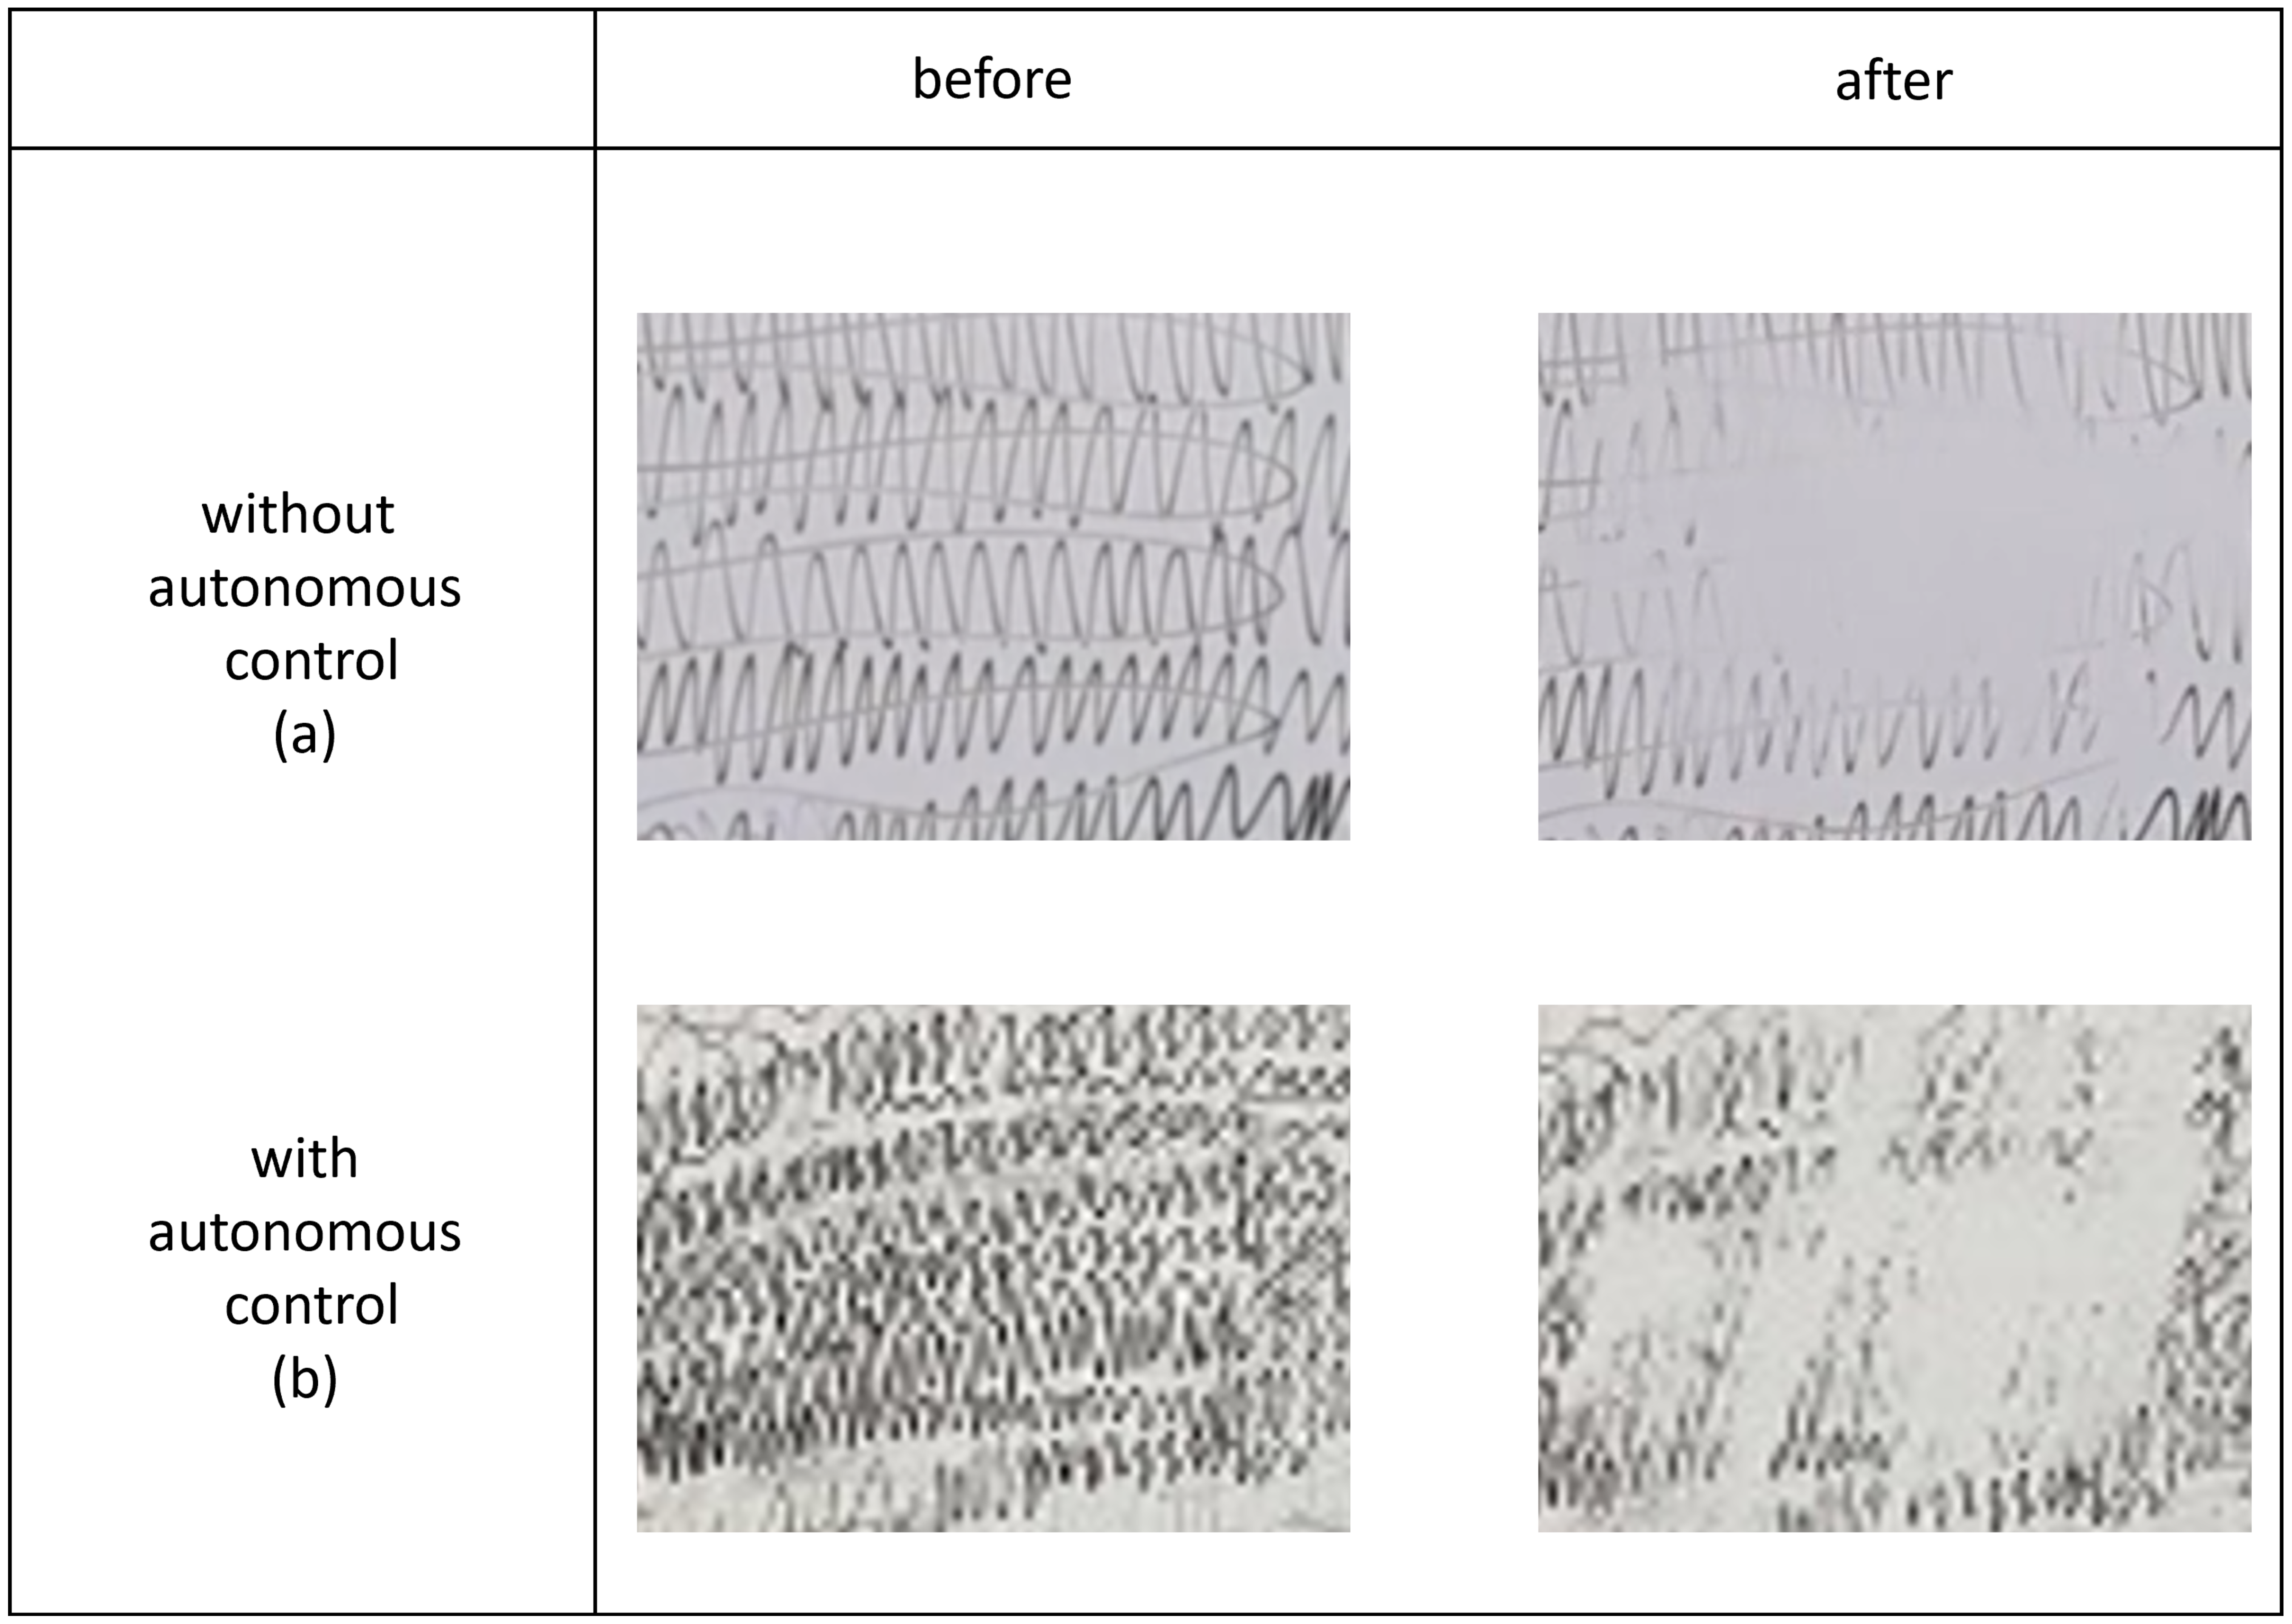
\includegraphics[width=0.8\columnwidth]{figs/wall_compare}
    \caption{Wall surface before and after cleaning}
    \label{fig:wall_compare}
\end{figure}

壁面の汚れについて,自律制御を用いなかった場合と用いた場合,どちらでも70\%程度インクを拭き取ることができている.
自律制御を用いた場合では,斜線状にインクが残っている箇所がある.
これは手先を押し付けて移動させたために,静止摩擦から動摩擦へ変化した際の摩擦力の急激な変化が発生し,手先工具が傾いてしまったためだと考えられる.
汚れを十分に拭き取るためには,押し付ける力を連続的に変化させることや,手先工具の形状を変更し工具が傾くことを防ぐことなどが必要である.

次に,手先を壁面に押しつける力制御について検証する.
壁面に垂直な方向の推定外力のプロットを図\ref{fig:hand_force_compare}にのせる.
この外力の反力が,ロボットが手先を壁面に押し付けている力だと言える.

自律制御を用いなかった場合(a)では,推定された外力はおよそ$\SI{-0.2}{\newton}$から$\SI{-2.0}{\newton}$の間で変動している.
一方で自律制御を用いた場合(b)では,推定された外力は目標力の反力$\SI{-2.0}{\newton}$と$\SI{-2.8}{\newton}$とおよそ一致している.
この結果から本研究で提案した力制御は目的を達成できていると言える.
ただし(b)の場合でも終盤には力は振動している.
これは壁面との摩擦によってロボットがyaw方向に回転してしまい,これを補正しようとする位置制御の結果,手先が壁面と垂直な方向に移動したためだと推察される.
壁面と垂直な方向だけでなく,摩擦の働く水平な方向についても考慮した制御が必要である.

最後に外力を補償し飛行を安定化させる制御について検証する.
実験中に飛行が安定していたかについては,ロボットの位置について,目標の指令値と実際の値の差分によって評価する.この差分が小さいほど飛行が安定であるとする.
実験中のロボットの位置の指令値と実値の差分をプロットしたものを図\ref{fig:pos_err_compare}にのせる.
壁面に平行な水平移動方向をx軸,壁面に垂直な押し付け方向をy軸,壁面に平行な鉛直方向をz軸としている.
y軸方向については壁面によって移動が制限されているため,評価の対象外とする.

自律制御を用いない場合(a)では$\SI{+0.25}{\meter}$近くまで差分が出ているのに比べ,自律制御を用いた場合(b)には$\SI{+0.20}{\meter}$未満まで抑えられている.
また(a)では差分はプラス方向にしか発生していないのに対し,(b)ではマイナス方向にも発生している.
これは壁面から受けた摩擦を補償しようとした結果であると推察される.
また,z軸方向に関しては,(a)(b)ともに$\SI{\pm0.05}{\meter}$の差分が発生しており,あまり改善は見られない.
これは今回の実験ではz軸方向にはロボットを移動させておらず,z軸方向の摩擦力が小さかったためだと考えられる.

\section{結論と今後の展望}
本研究では,多関節飛行ロボットを操縦するためのデバイスと,作業中の外力を補償し飛行を安定させながら目標の手先力を発揮するための自律制御からなる遠隔操縦システムを提案した.
提案したデバイスによって,多関節飛行ロボットのベースと関節の自由度を同時に操縦することが可能になった.また,ロータの偏向角を制御する自律制御によって,より安定して手先力を用いたタスクを行えるようになった.
そして壁面の清掃実験を通して,提案した遠隔操縦システムの有用性を検証した.

手先を押し付ける力のみでなく,摩擦力まで考慮した自律制御を構築することで,より安定してタスクを行うことができると考えられる.また,作業中にロボットが受ける外力を,操縦者に力覚的にフィードバックすることで,より円滑にタスクを行うことができるだろう.
そして将来的には,提案した遠隔操縦システムを,様々な環境で様々なタスクを行えるようなシステムに発展させることを目指す.

\begin{figure}[t]
    \centering
    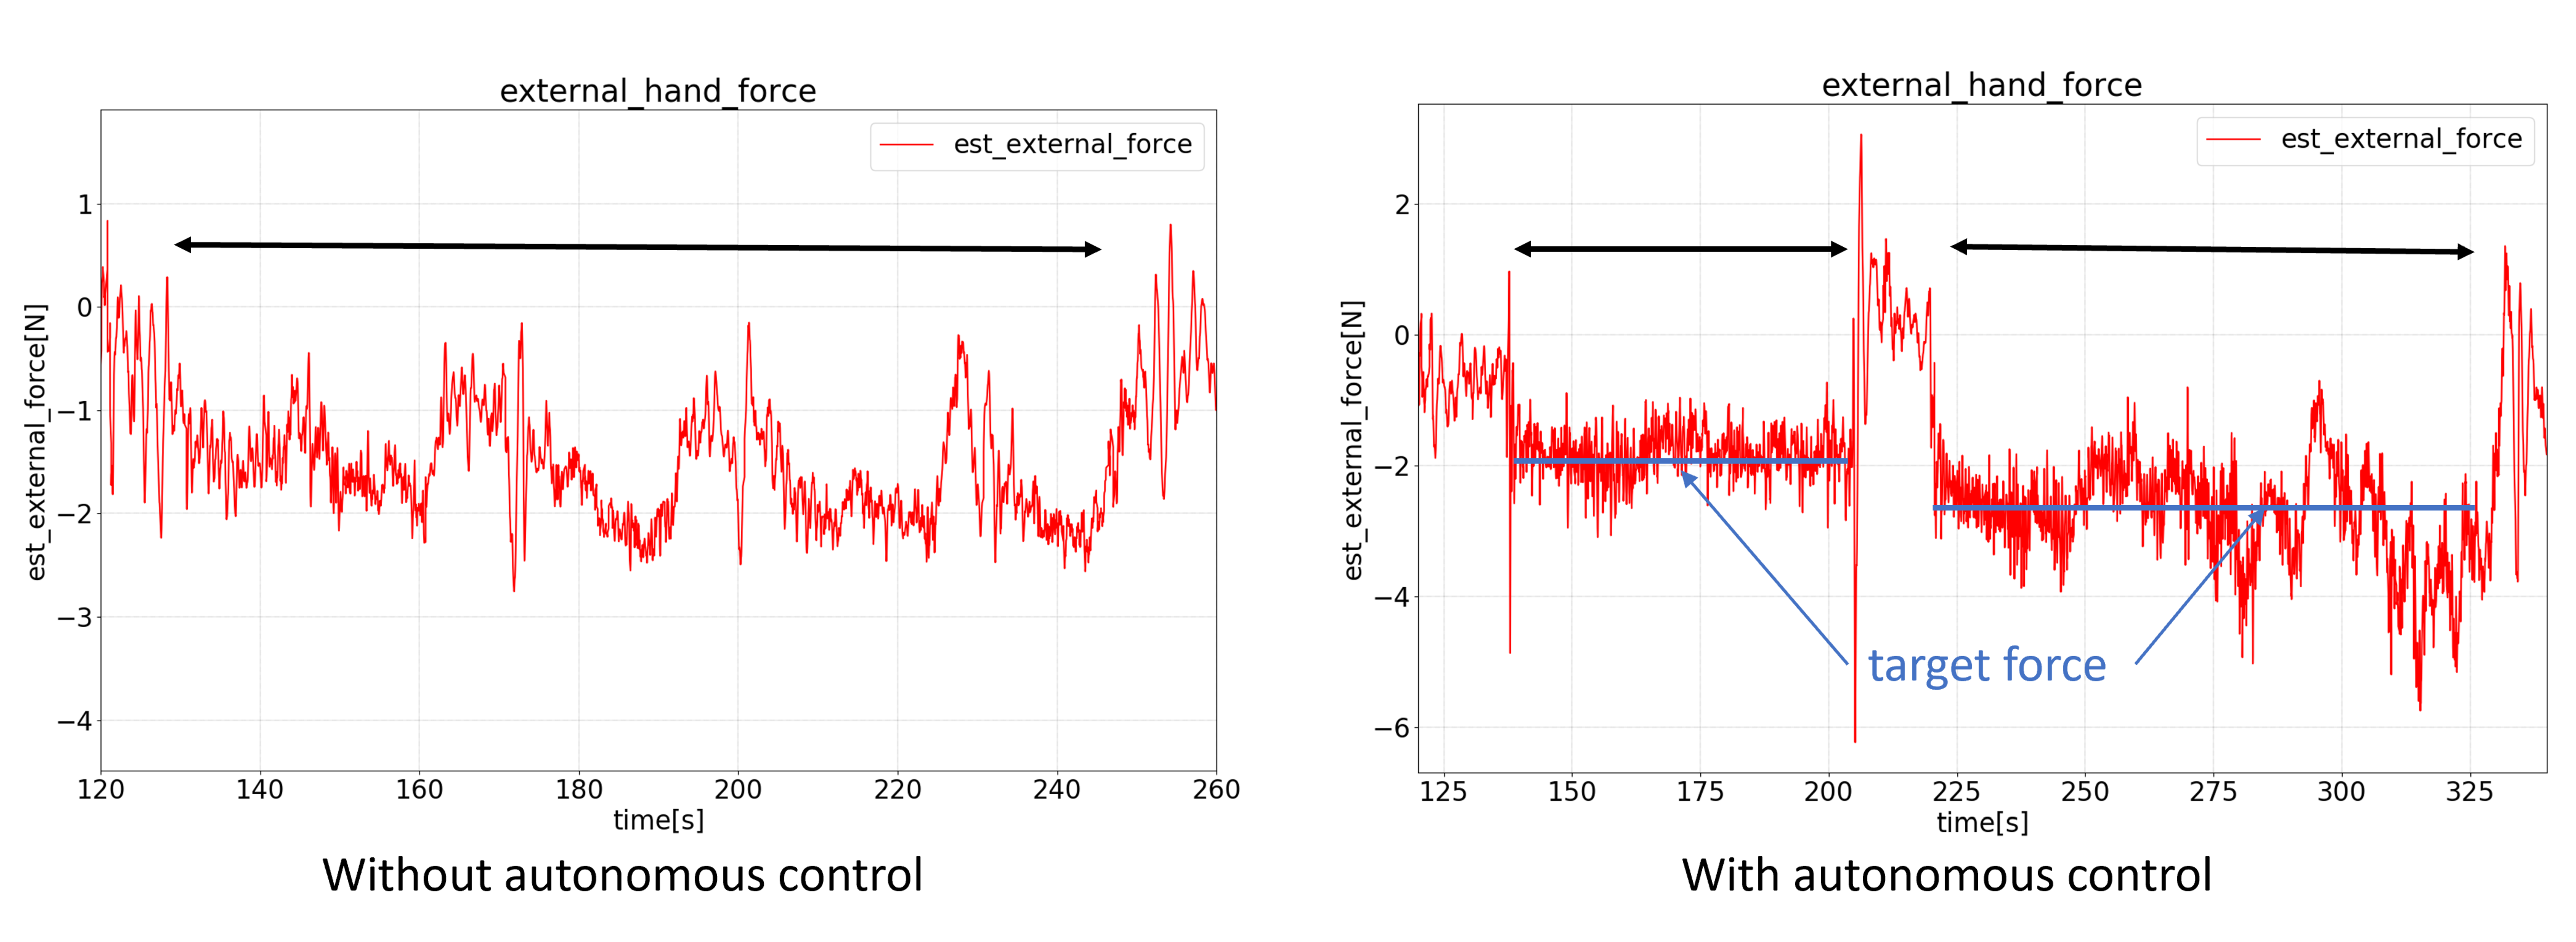
\includegraphics[width=1.0\columnwidth]{figs/hand_force_compare}
    \caption{Estimated end-effector's pressing reaction force}
    \label{fig:hand_force_compare}
\end{figure}

\begin{figure}[t]
    \centering
    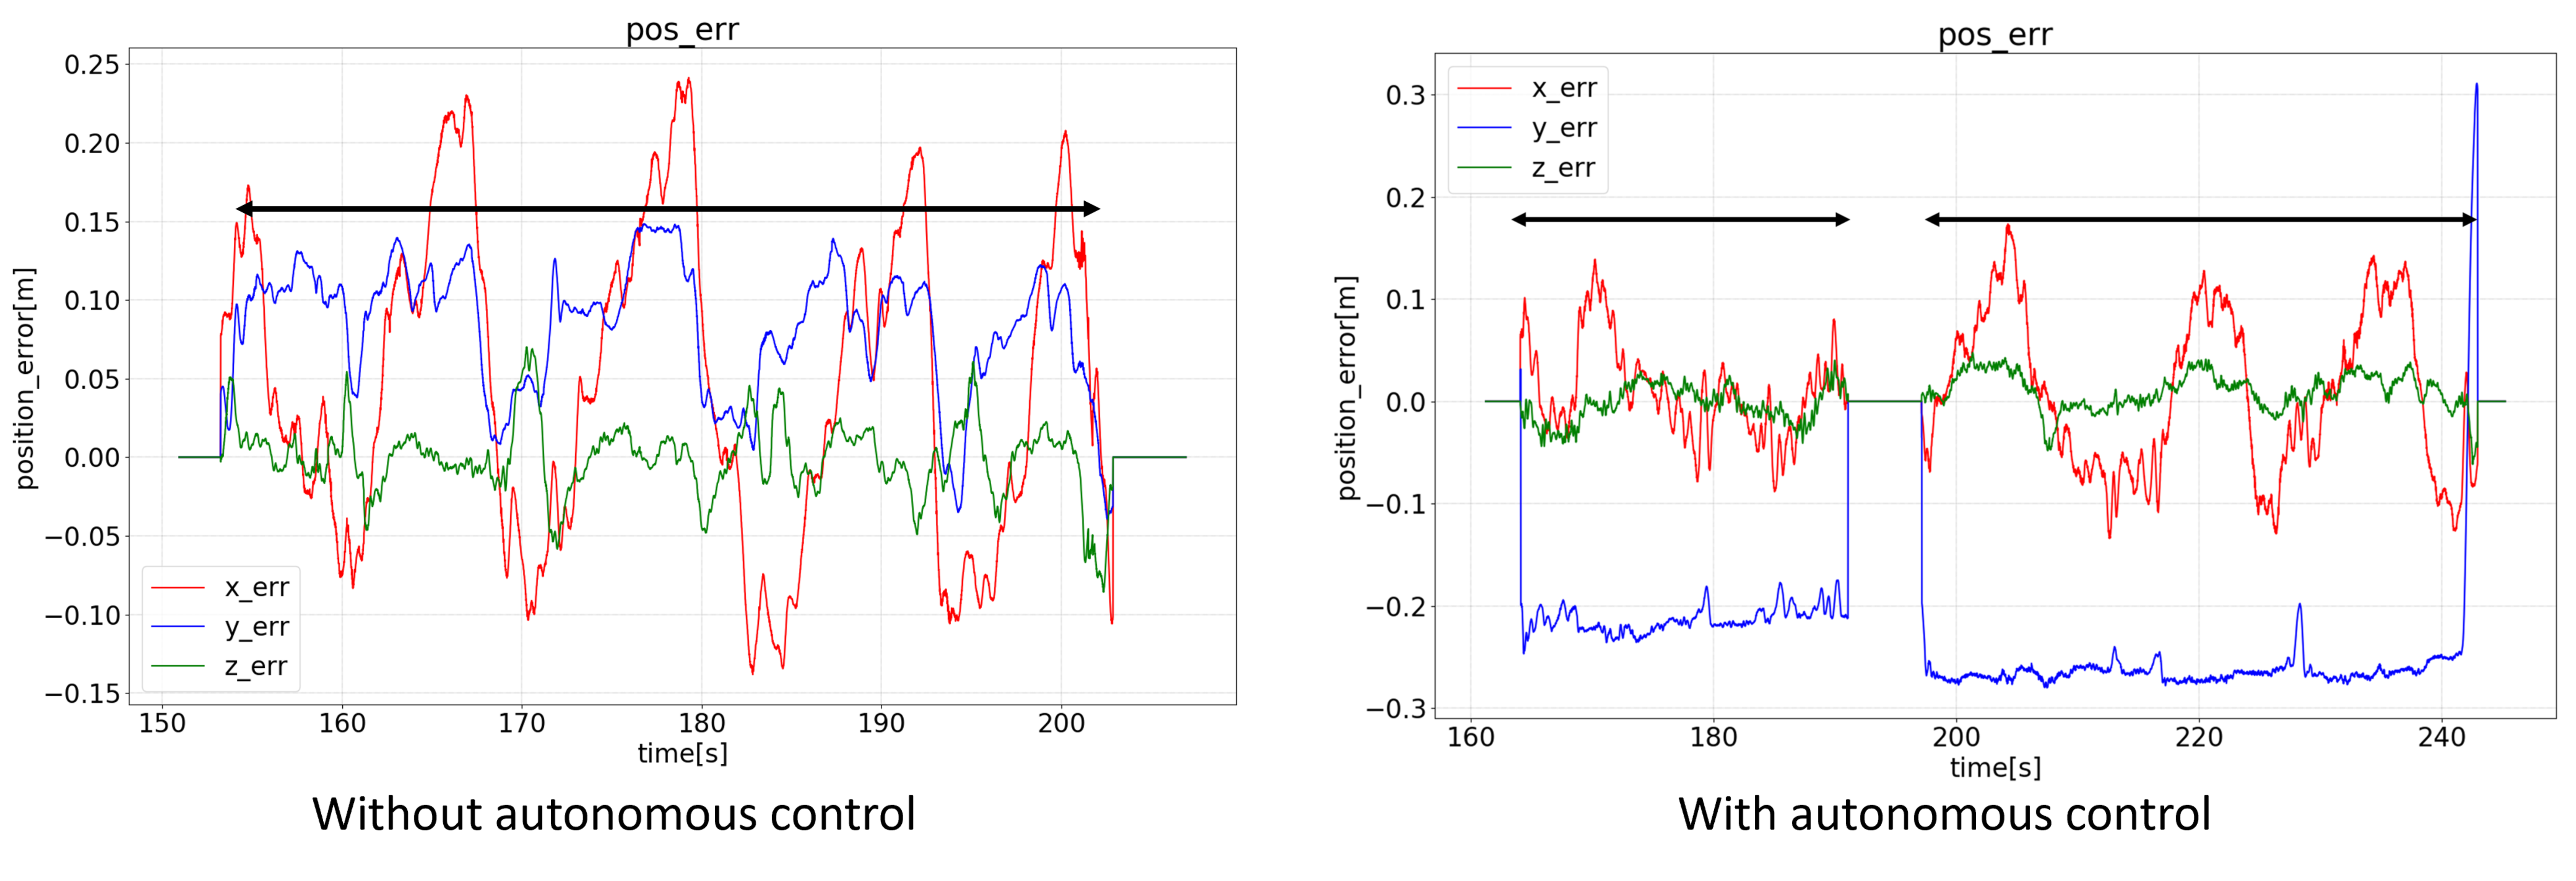
\includegraphics[width=1.0\columnwidth]{figs/pos_err_compare}
    \caption{Difference between commanded and actual position values}
    \label{fig:pos_err_compare}
\end{figure}

\footnotesize
% \begin{thebibliography}{99}
\bibliographystyle{junsrt}
\bibliography{bib.bib}
% \bibitem{Shinjuku98}
% 新宿大五朗,渋谷次郎,東京 学,``キャスティングマニピュレーションに関する研究(第1報,可変長の紐状柔軟リンクを有するマニピュレータの提案とそのスイング制御法)'',{\it 機論C編}, vol.64-626, pp.3854--3861, 1998.

% \bibitem{Shinjuku99}
% Shinjuku, D., Shibuya, J. and Tokyo, M., ``Swing Motion Control of Casting Manipulation,'' {\it IEEE Control Systems}, vol.19-4, pp.56--64, 1999.

% \end{thebibliography}

\normalsize
\end{document}
